% Week 3 实验周报 —— 编译方式:XeLaTeX
\documentclass[11pt]{ctexart}
\usepackage[a4paper, margin=2.5cm]{geometry}
\usepackage{amsmath}
\usepackage{booktabs}
\usepackage{graphicx}
\usepackage{hyperref}
\usepackage{enumitem}
\setlist{nosep}

\title{\textbf{Chooser Option 定价项目 —— 第 3 周实验报告}\\
\large Original BSM Model Replication}
\author{佟铸城 (Zhucheng Tong)}
\date{2026 年 8 月 4 日}

\begin{document}
\maketitle

\section{本周目标}
完成 Week 3 三项交付物:(1) 可运行的 BSM chooser 定价代码;(2) 模型验证脚本(与论文结果对照);(3) 参数配置文件。交付形式按导师要求采用纯 Python 脚本(不使用 Jupyter Notebook)。

\section{完成工作}
\begin{enumerate}
  \item \textbf{定价模块}(\texttt{src/models/}):BSM vanilla 定价(\texttt{bsm.py});chooser 闭式解\textbf{两种独立实现}——Rubinstein 分解法(call$(K,T_2)$ + $e^{-q\tau}$份 put$(K^*,t_1)$,$K^*=Ke^{-(r-q)\tau}$)与 Hull 直接公式法,互为正确性校验;
  \item \textbf{蒙特卡洛引擎}:两段 GBM 模拟,支持\textbf{双选择规则}(理性规则 $\max(C,P)$ vs 论文的 moneyness 规则 $S_{t_1}>K$);采用\textbf{条件 MC}(选择日期权价值用解析式而非继续模拟)与对偶变量降方差;另实现终值模拟版作独立核对;
  \item \textbf{分析脚本交付}(\texttt{analysis/week3/}):\texttt{01\_bsm\_chooser\_model.py}(模型实现与推导讲解、内置正确性断言)、\texttt{02\_model\_validation.py}(收敛性表、路径表、敏感性、规则对比),均可从项目根目录直接运行,分节打印全部验证结果;
  \item \textbf{参数配置文件}:\texttt{configs/paper\_params.json}(论文 Table 2:$S_0=156.7$, $K=150$, $r=0.15\%$, $\sigma=28.2\%$, $q=2.33\%$, $t_1=0.5$, $T_2=1$)。
\end{enumerate}

\section{核心结果}
\begin{center}
\begin{tabular}{lr}
\toprule
\textbf{量} & \textbf{数值} \\
\midrule
Chooser 闭式解(论文参数) & \textbf{\$29.1299} \\
两种闭式解实现差异 & $7.1\times10^{-15}$(浮点精度) \\
Vanilla call / put($K$=150, $T_2$=1) & \$18.6890 / \$15.3731 \\
Straddle(call+put) & \$34.0621 \\
MC 理性规则(100 万路径) & \$29.1426 $\pm$ 0.0165 \\
MC moneyness 规则(同种子配对) & \$29.1249 \\
\bottomrule
\end{tabular}
\end{center}

经济学排序 $\max(C,P) < \text{chooser} < \text{straddle}$ 成立:相对只买 call 的灵活性溢价 \$10.44,相对 straddle 的折价 \$4.93(``推迟选择''比``两个都买''便宜的部分)。

\section{与论文的对照}
\begin{enumerate}
  \item \textbf{对照标准的说明}:论文未报告明确的 chooser 价格数字(第 1 周周报已指出),故复现以\textbf{结构性标准}为准:(a) Table 3 路径表逻辑——已复现(10 条示例路径,payoff 计算逐行一致);(b) Fig.3--6 敏感性方向——全部复现(见图~\ref{fig:sens}):$\sigma\uparrow$ 双腿同涨、$K\uparrow$ call 跌 put 涨、$r\uparrow$ call 涨 put 跌、$q$ 反向;
  \item \textbf{超出论文的增量之一($t_1$ 敏感性,论文自认的未竟工作)}:chooser 价值随 $t_1$ 单调上升,两端点有清晰经济含义——$t_1\to0$ 退化为 $\max(C,P)$(立刻选定),$t_1\to T_2$ 收敛到 straddle(永不放弃任一方向);
  \item \textbf{超出论文的增量之二(其选择规则的代价量化)}:论文在 $t_1$ 用 $S_{t_1}$ vs $K$ 决定 call/put,理性规则应比较期权价值,无差异临界点在 $S^*=Ke^{(q-r)\tau}$ 而非 $K$。同种子配对估计显示:论文参数下($r=0.15\%$)该规则仅低估 \textbf{6.1 bp}——因为 $r\approx q$ 使 $S^*\approx K$;但当 $r=10\%$ 时代价放大到 \textbf{60 bp}。结论:论文的简化在 2021 年零利率环境下无害,但不可移植到高利率状态——这对第 4 周用 2022--2024 加息期数据做评估是一个直接相关的预警。
\end{enumerate}

\begin{figure}[h!]
\centering
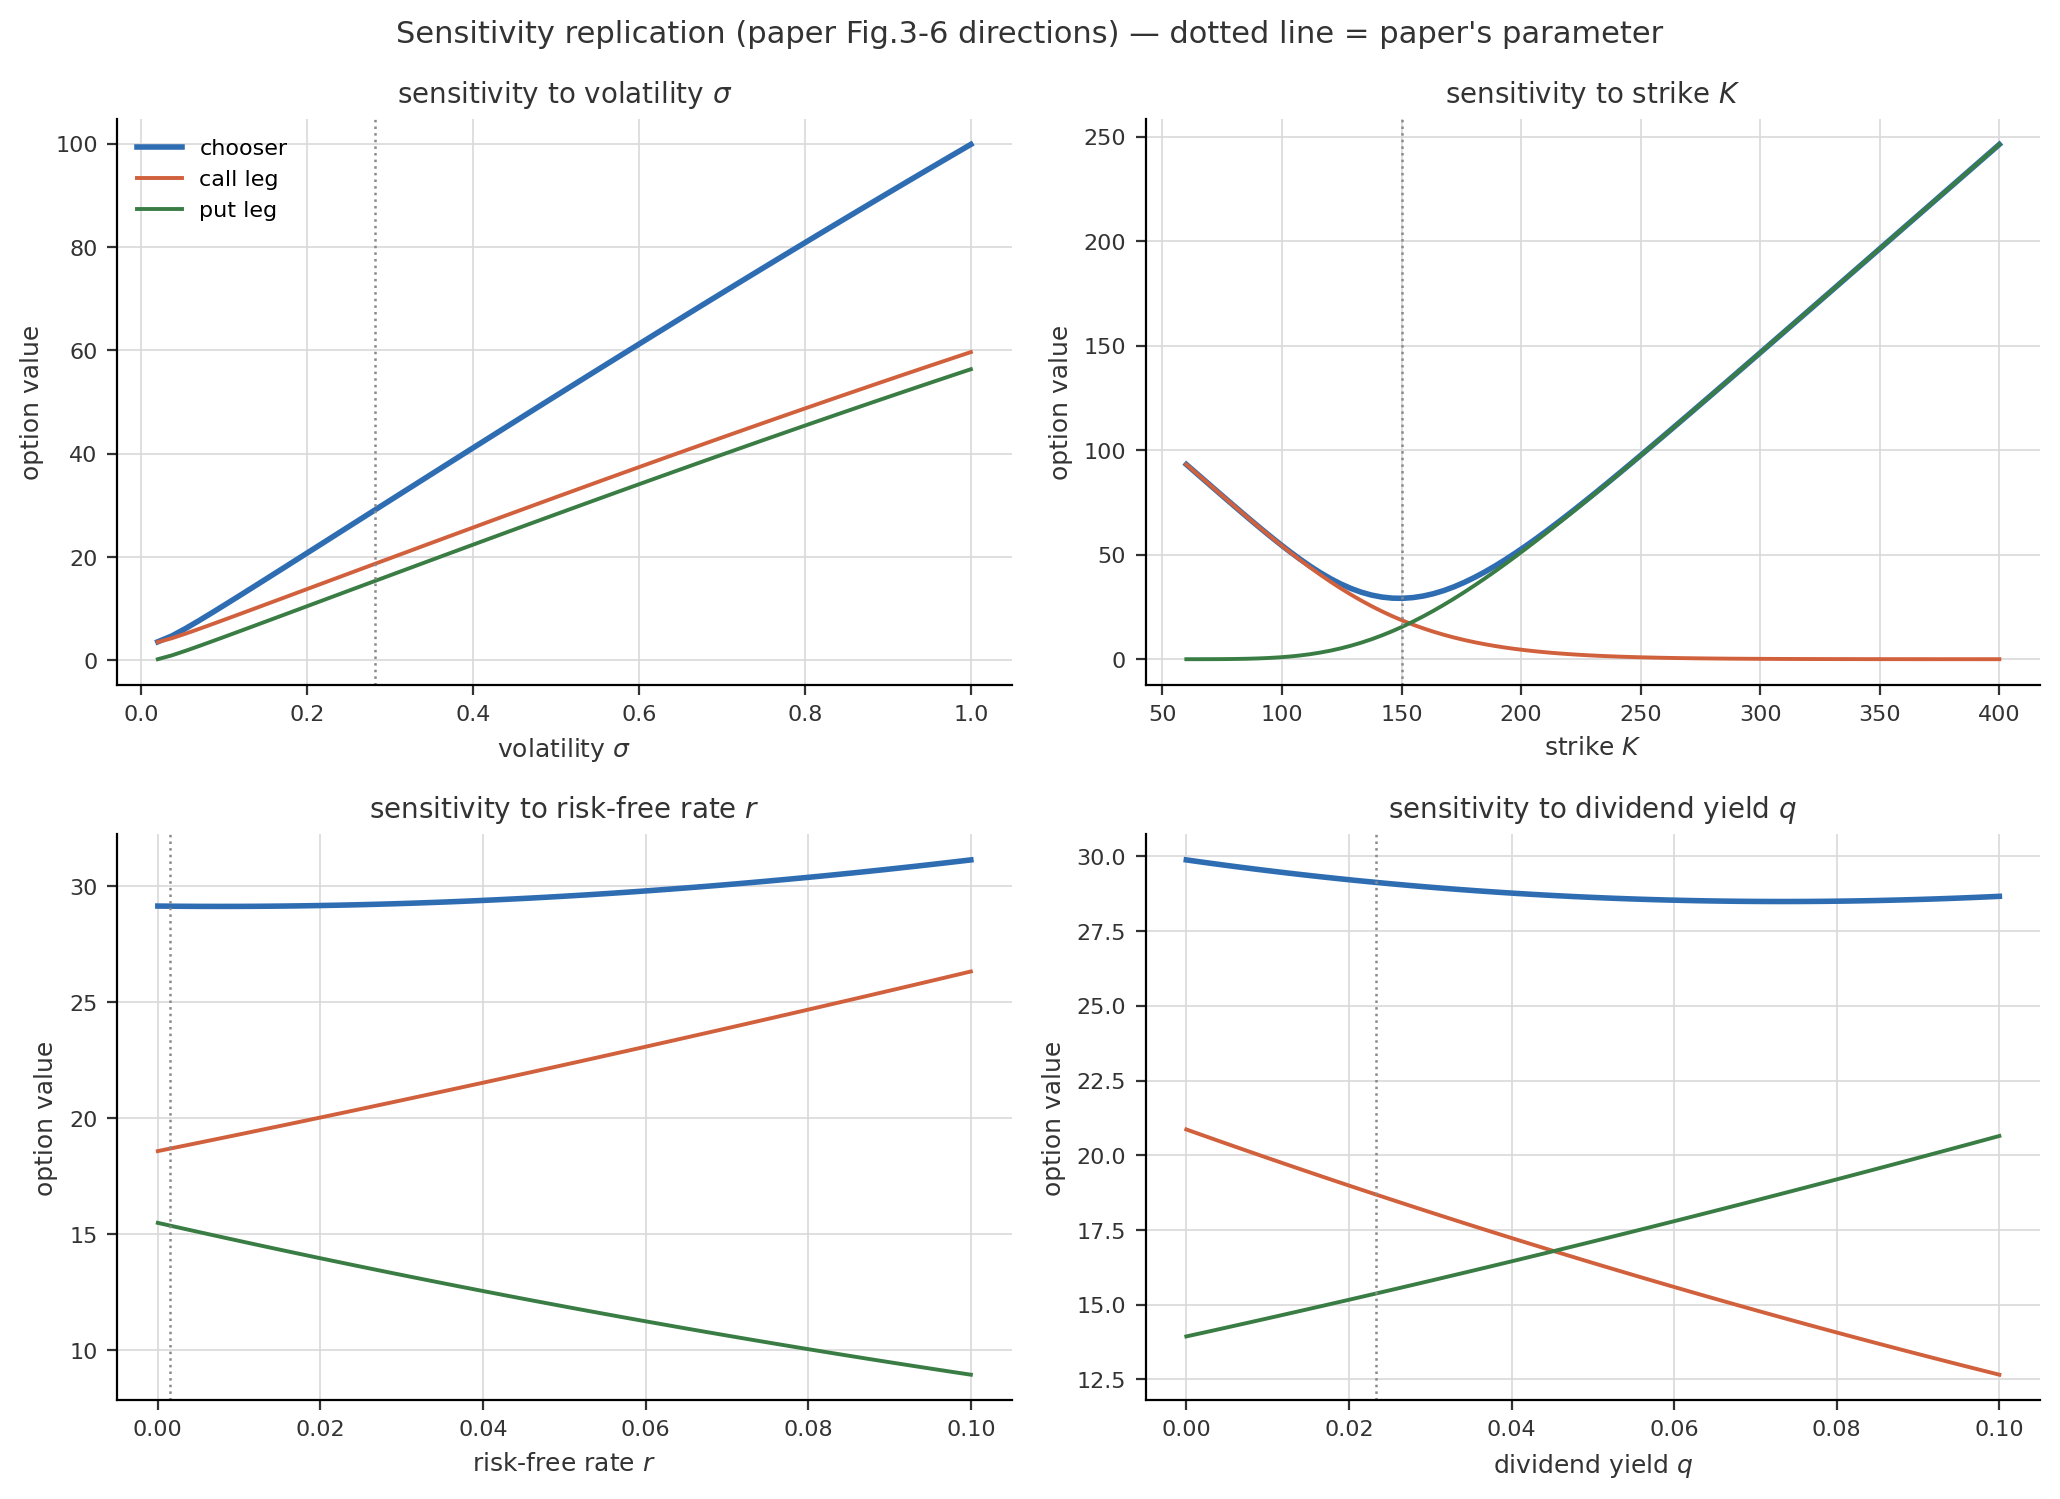
\includegraphics[width=0.94\textwidth]{../../docs/week3/figures/sensitivity_panels.png}
\caption{敏感性复现($\sigma$/$K$/$r$/$q$,虚线为论文参数点);chooser 对 $K$ 呈 U 形、谷底近远期价}
\label{fig:sens}
\end{figure}

\begin{figure}[h!]
\centering
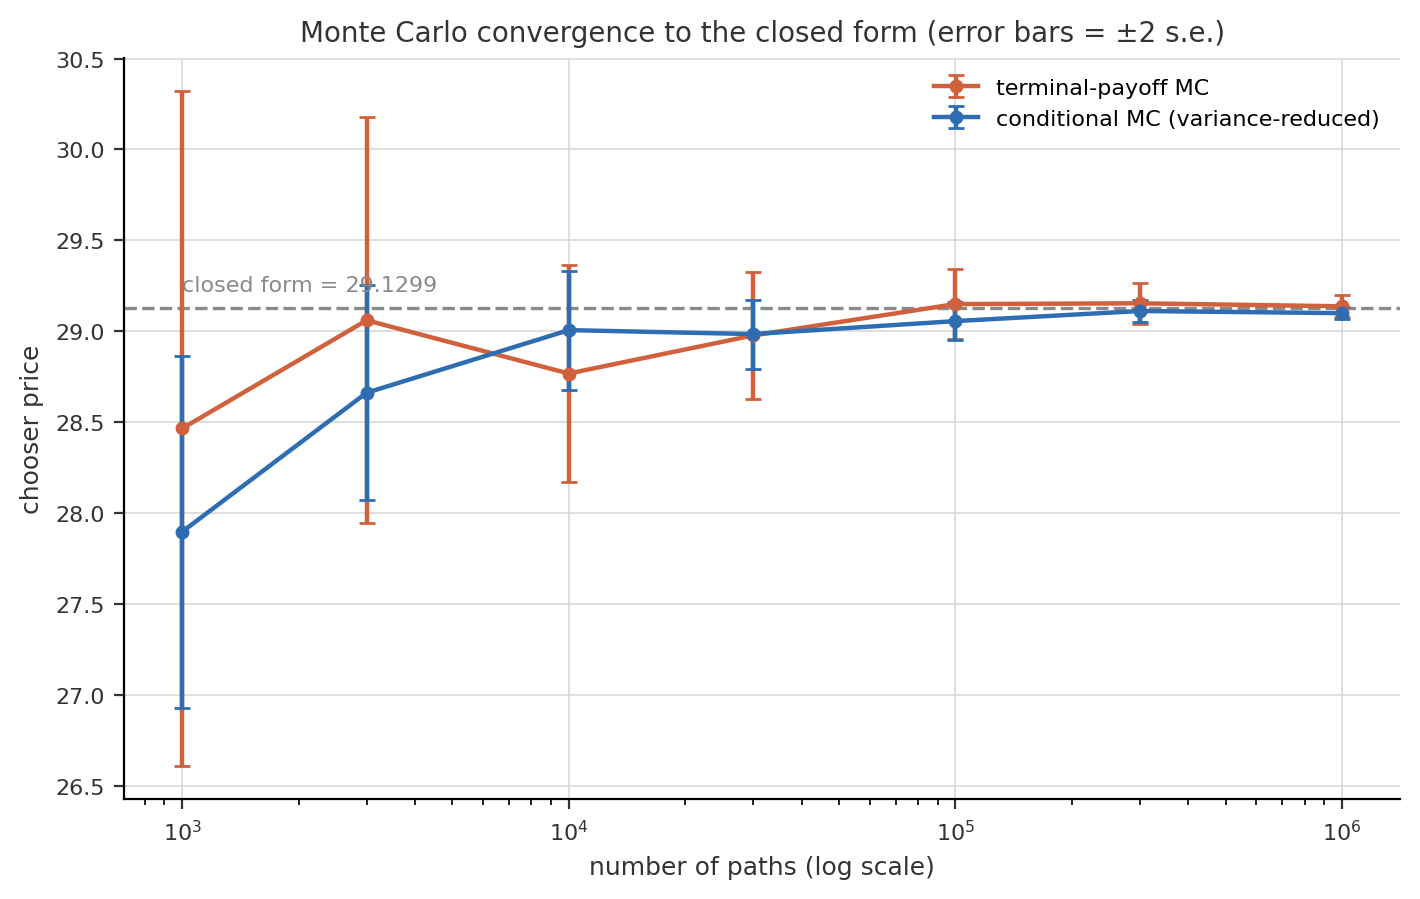
\includegraphics[width=0.62\textwidth]{../../docs/week3/figures/convergence.png}
\caption{MC 收敛性:两种估计量均以 $1/\sqrt{n}$ 收敛于闭式解;条件 MC 标准误约为终值模拟的一半}
\end{figure}

\section{实验记录}
条件 MC 的降方差效果:同等路径数下标准误约为终值模拟的 54\%(等效于路径数 $\times$3.4),原理是把第二段模拟噪声完全用解析式消除——延续第 2 周``方差缩减是必需品''的工程原则。规则对比使用同种子(common random numbers)配对,使 0.0177 的微小差距在统计上可分辨。

\section{下周计划(Week 4:基线模型性能评估)}
\begin{enumerate}
  \item 以 MC 为基准正式化验证框架(导师指定方案),输出 MAE/RMSE 收敛指标;
  \item 用真实数据滚动校准参数($\sigma$ 用滚动已实现波动率、$r$ 用期限匹配国债、$q$ 用 TTM 股息率),在 2018--2024 全窗口逐日定价;
  \item 按波动状态分组(恐慌标记/VIX 分位)分析 BSM 常数波动率假设的失效模式,重点考察 2020-03 与 2022 加息期;
  \item 建立基线性能文档,为第 5--6 周 ML 对比设定基准。
\end{enumerate}

\end{document}
